% Generated by experiments/icpc/make_result_figs.py from committed results. Do not edit by hand.
\documentclass[border=2pt]{standalone}
\usepackage[T1]{fontenc}\usepackage{newtxtext,newtxmath}\usepackage[varqu,scaled=0.95]{zi4}
\usepackage{pgfplots}\pgfplotsset{compat=1.18}
\definecolor{cblue}{HTML}{0072B2}\definecolor{cver}{HTML}{D55E00}\definecolor{cora}{HTML}{E69F00}
\definecolor{cgreen}{HTML}{009E73}\definecolor{cgrey}{HTML}{999999}\definecolor{csky}{HTML}{56B4E9}\definecolor{cpurple}{HTML}{7E57C2}
\pgfplotsset{every axis/.append style={font=\footnotesize, tick label style={font=\scriptsize},
  label style={font=\footnotesize}, legend style={font=\scriptsize, draw=none, fill=none},
  axis lines*=left, ymajorgrids, grid style={black!8}}}
\begin{document}
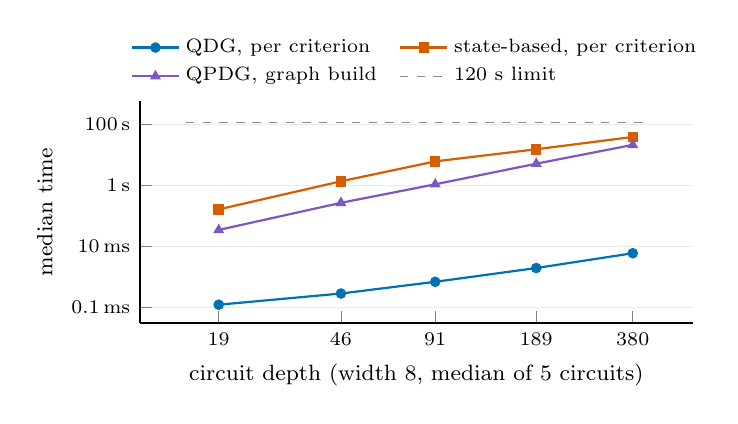
\begin{tikzpicture}\begin{axis}[width=8.6cm, height=4.4cm, xmode=log, ymode=log, log basis x=2,
 xtick={19,46,91,189,380}, xticklabels={19,46,91,189,380}, xlabel={circuit depth (width 8, median of 5 circuits)},
 ylabel={median time}, ymin=3e-5, ymax=600, ytick={1e-4,1e-2,1,100}, yticklabels={0.1\,ms,10\,ms,1\,s,100\,s},
 legend style={at={(0.5,1.02)}, anchor=south, legend columns=2, /tikz/every even column/.append style={column sep=6pt}}, legend cell align=left]
\addplot[cblue, thick, mark=*, mark size=1.5pt] coordinates {(19,0.000120) (46,0.000280) (91,0.000680) (189,0.001930) (380,0.005925)};
\addplot[cver, thick, mark=square*, mark size=1.5pt] coordinates {(19,0.164000) (46,1.377700) (91,6.232250) (189,15.596600) (380,39.606850)};
\addplot[cpurple, thick, mark=triangle*, mark size=1.5pt] coordinates {(19,0.034600) (46,0.269600) (91,1.097100) (189,5.226600) (380,21.717200)};
\addplot[black!45, dashed, domain=15:420] {120};
\legend{{QDG, per criterion},{state-based, per criterion},{QPDG, graph build},{120 s limit}}
\end{axis}\end{tikzpicture}
\end{document}
